\section{Evaluation}\label{sec:eval}
In this chapter, we evaluate the presented approaches using the trained models from ~\autoref{sec:multi-task-ft} and \autoref{sec:single-task-ft} to extract event logs from Patient Journeys. In order to properly compare the fine-tuned models and the base model, we first introduce the metrics we use. Second, we describe the evaluation process. Third, we present our results for each model, each task and each of the task's metrics individually.\\
We evaluate the extracted event logs by comparing them to ground truths and determining their differences. This is one of a few options already established in the academic context~\cite{latif_fine-tuning_2024}.

\subsection{Metrics}\label{sec:metrics}
In \autoref{sec:multi-task-ft}, we describe the process of fine-tuning a model to perform multiple related tasks. We evaluate each of these tasks individually. The model trained in \autoref{sec:single-task-ft} performs only the task \quotes{Activity Labeling}, so we use the metric described in \autoref{sec:activity_metrics} for this model as well.

\subsubsection{Activity Labelling Metrics}\label{sec:activity_metrics}
There are already established metrics in the process mining sector that we can use to determine if an event log is of good quality regarding activities. \cite{van_der_aalst_process_2016, carmona_conformance_2018} propose three categories an activity can have. We use similar categories for the activity labels.\\
It is worth noting that determining if one activity label from the evaluated event log and one from the ground truth are indeed the same activity label is challenging. As discussed in \autoref{sec:tracex}, the possible activity labels are not predetermined. Instead, the model that extracts them chooses the exact phrasing. This means two activity labels can be syntactically different but still describe the same activity. For the purpose of this evaluation, we define two activity labels as identical if they are semantically very similar.
\paragraph{Missing Activity} An activity is missing if it is featured in the ground truth but not in the evaluated event log. 
\paragraph{Unexpected Activity} An activity is unexpected if it is featured in the evaluated event log but not in the ground truth. This can either mean the model hallucinated an activity or that the activity is featured in the Patient Journey but is not relevant and, therefore, not listed in the ground truth event log.
\paragraph{Wrong Order} Two activities are in the wrong order if both are featured in the ground truth and the evaluated event log, but their order of appearance is interchanged. In our case, the order of activities is defined by their start timestamp. This means two activities $A_1 \text{ and } A_2$ are in the wrong order if they appear in the order $A_1,A_2$ in the ground truth and in order $A_2, A_1$ in the evaluated event log.\\\\
As this is a comparative analysis, the value we use from this metric is the percentage of errors in each of the mentioned categories – Missing Activity, Unexpected Activity, and Wrong Order. This way, the number of errors is relative to the number of activities in each Patient Journey.

\subsubsection{Event Type Classification Metric}\label{sec:eventtype_metric}
We use a set of event types, so each pair is mutually exclusive. This means that there is exactly one correct event type for every activity in the ground truth. This fact reduces this metric to two possible results per event type: \emph{True} and \emph{False.}\\
The value we use from this metric is the percentage of \verb|True| and \verb|False| values respectively. This way, the number of errors is relative to the number of activities in each Patient Journey.\\
Possible event types are: Symptom Onset, Symptom Offset, Doctor Visit, Hospital Admission, Hospital Discharge, Diagnosis, Treatment, Medication, Lifestyle Change and Feelings.

\subsubsection{Timestamp Extraction Metric}\label{sec:time_metrics}
Similar to the event type metric, a timestamp can be either extracted correctly or incorrectly, resulting in \verb|True| or \verb|False| when evaluated. In order to adhere to the commonly used standard in event logs, which is also required to produce valid XES files, the timestamps are in the format \verb|YYYY-MM-DD|. In many cases, including the sample Patient Journeys we use in the evaluation, Patient Journeys do not contain time information this precise. Most of the time, specifications are relative and vague. For this evaluation, we define a timestamp to be extracted correctly if the date is plausible in the context of the Patient Journey. For an activity described to have happened on \quotes{some day in April…}, any timestamp between 01.~April and 30.~April would be correct. This is unless other time-related information further specifies the timeframe in which an activity must have happened. Let $A_1$ be an activity that happens before activity $A_2$ and $t_2=$ \verb|2024-04-15| be the timestamp for $A_2$. If $A_1$ is specified as \quotes{some day in April…}, only timestamps between 01.~April and 14.~April are correct. The same goes for \quotes{as the weeks progressed}, \quotes{later that year} and similar phrases. As long as an extracted timestamp is correct relative to all other information given in the Patient Journey and is as precise as the text provides, it is deemed correct.\\
Start and end timestamps can be correct or incorrect, independent of each other. The value we use from this metric is the percentage of \verb|True| and \verb|False| values respectively. This way, the number of errors is relative to the number of activities in each Patient Journey.

\subsection{Evaluation Process}\label{sec:eval_process}
In this chapter, we describe the process of evaluating the models trained in \autoref{sec:multi-task-ft} and \autoref{sec:single-task-ft} using the metrics proposed in \autoref{sec:metrics}.\\
In order to evaluate the quality of the extraction performed by the various models, we need Patient Journeys to extract event logs from. First, we assemble a collection of Patient Journeys that pose different challenges. They are listed in full length in the appendix at \ref{apx:pjs}. They include well-structured descriptions of consecutive events and explicitly stated timestamps, but also implied activities and events with strong temporal relations that are not easily understood without considering a big context window. In short, the reference Patient Journeys provide diverse challenges, featuring both easy and hard-to-extract information.\\
We conduct comparative analyses between LLM models. To make these as fair and deterministic as possible, the next step is to create ground truths for every Patient Journey and every task performed on them. They are listed in the appendix at \ref{apx:ground_truths}. We later on use the same Patient Journeys and respective ground truths for all models.\\
We perform the extraction itself using the TracEX pipeline. To address the dependency of the Event Type Classification step detailed in \autoref{sec:back}, we inject the activities from the ground truth into the pipeline before executing that step. This ensures that no previous step affects the results of the extraction in an uncontrolled way.\\\\
The extraction uses LLMs, which are non-deterministic by design. Due to that fact, the results vary between executions, even with the same input. To solve this issue, we perform each execution multiple times and use the mean of all values between the executions for the evaluation. All datasets without the mean calculation are archived in the aforementioned repository, together with the Patient Journeys.\\\\
As mentioned in \autoref{sec:tracex}, TracEX uses few-shot prompts for every task we examine in this thesis. The fine-tuned models perform all tasks without the additional examples in the few-shot prompts since the training data should suffice to convey what is demanded from the model.\\
% Every Journey will be preprocessed~\ref{sec:tracex} before every extraction, regardless of model or task.

\subsubsection{Evaluating Activity Labelling}\label{sec:eval_activity}
In this chapter, we describe the process of evaluating the activity label extraction capabilities of LLMs using the TracEX pipeline. Our approach primarily involves the use of automated processes. The following algorithm is implemented similarly in the Trace Testing Environment of TracEX.\\\\
For each activity in the event log, we look for a matching activity in the ground truth. We limit the number of activities to ±2 from the current activity to prevent false positives. We assume the activities are sorted by start timestamp. So, an activity from the event log with index five would be compared to the activities with index three to seven from the ground truth. As mentioned earlier, two activity labels must be semantically very similar to be considered a match. This is done by prompting GPT-4, a much more capable model than GPT-3.5 Turbo, to rate the semantic similarity. The response from the OpenAI API also includes a \verb|logprobs| parameter that indicates how confident the model is in its response. If no activity from the ground truth matches, we consider this activity \emph{unexpected}. If exactly one activity from the ground truth is a match, that activity is considered correctly extracted. If multiple activities from the ground truth are matched, we use the one with the highest confidence score and consider the activity correctly extracted.  All activities from the ground truth that remain without a match are considered \emph{missing}. Two activities from the event log with a matching activity in the ground truth each, but whose order is interchanged in the event log compared to the ground truth, are counted as a \emph{wrong order} error.\\
The evaluation is automated to a large degree – but not perfect. We manually check every evaluation and adjust the three metrics' results accordingly. The values for each metric can be checked for every run of the extraction pipeline for every model and every Patient Journey in the repository.

\subsubsection{Evaluating Event Type Classification}\label{sec:eval_event_type}
The metric described in \autoref{sec:eventtype_metric} can be evaluated with a simple string comparison. The classified event types for all activities can be correct or incorrect. Because we injected the activities from the ground truth into the pipeline, we can compare them directly. The value for each index in the extracted event log must be identical to the value at the same index in the ground truth.

\subsubsection{Evaluating Timestamp Extraction}\label{sec:eval_time}
Time-related information in real-world Patient Journeys is, in many cases, so rare and vague that it is hard to determine a timestamp perfectly, even for a human. For this reason, we evaluate this metric completely manually, as we do not want to rely on LLMs to do it. The metric described in \autoref{sec:time_metrics} is designed to leave room for interpretation since we believe interpreting the time-related information in a Patient Journey as a human is the best way to derive concrete timestamps correctly and with the certainty needed in an evaluation.

\subsection{Presentation of Results}\label{sec:results}
In this chapter, we present and discuss the results we achieved by applying the metrics defined in \autoref{sec:metrics} to the event logs created by the models trained in \autoref{sec:multi-task-ft} and \autoref{sec:single-task-ft}.\\
We first showcase the multi-task fine-tuned model and, secondly, the single-task fine-tuned model, comparing each to GPT-3.5 Turbo. We perform the extraction on the Patient Journeys listed in \ref{apx:pjs}.

\subsubsection{Multi-Task Fine-Tuned Model}\label{sec_eval_multi}
We present the results for every task performed by the model in the following order: First, we showcase the performance in labelling activities, followed by classifying event types of activities, and lastly, extracting timestamps for activities.

\begin{figure}[p]
  \centering
  \captionsetup{belowskip=0pt,aboveskip=0pt}
  \subfigure[Patient Journey No. 1]{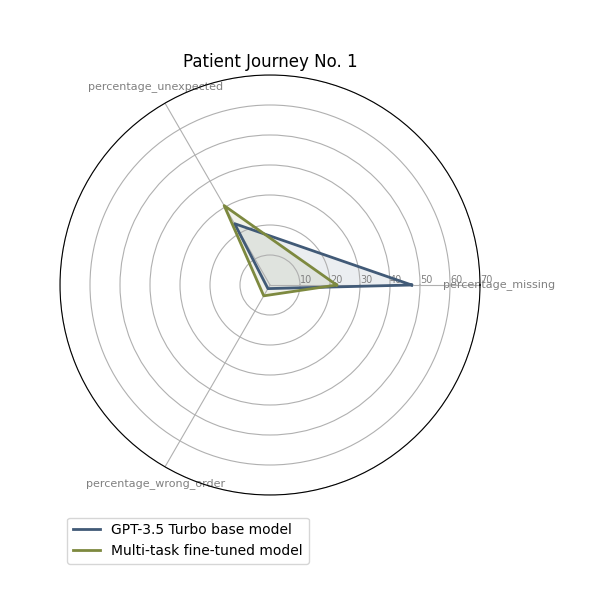
\includegraphics[width=0.3\textwidth]{bachelor_thesis/images/activites_pj1.png}}
  \subfigure[Patient Journey No. 2]{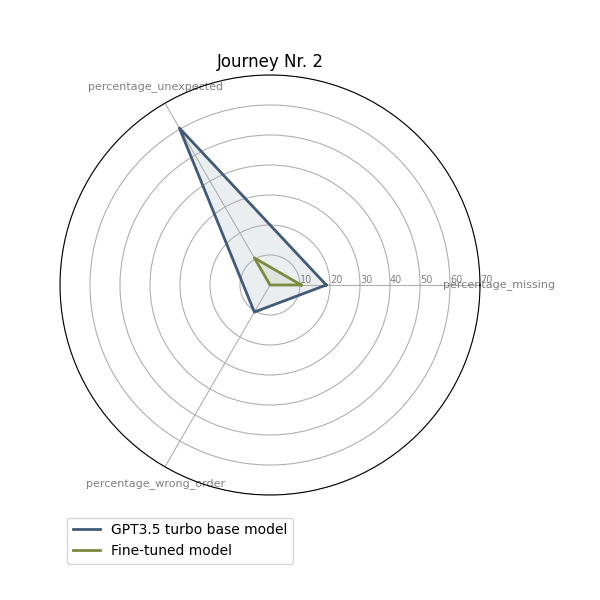
\includegraphics[width=0.3\textwidth]{bachelor_thesis/images/activites_pj2.png}}
  \subfigure[Patient Journey No. 3]{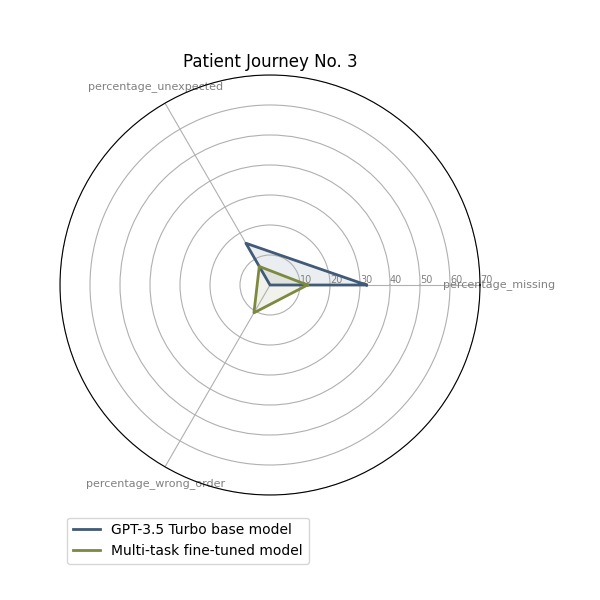
\includegraphics[width=0.3\textwidth]{bachelor_thesis/images/activites_pj3.png}}
  \subfigure[Patient Journey No. 4]{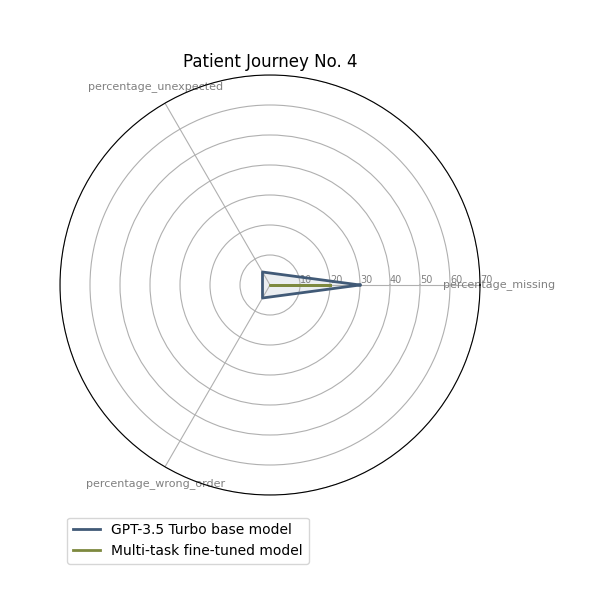
\includegraphics[width=0.3\textwidth]{bachelor_thesis/images/activites_pj4.png}}
  \subfigure[Patient Journey No. 5]{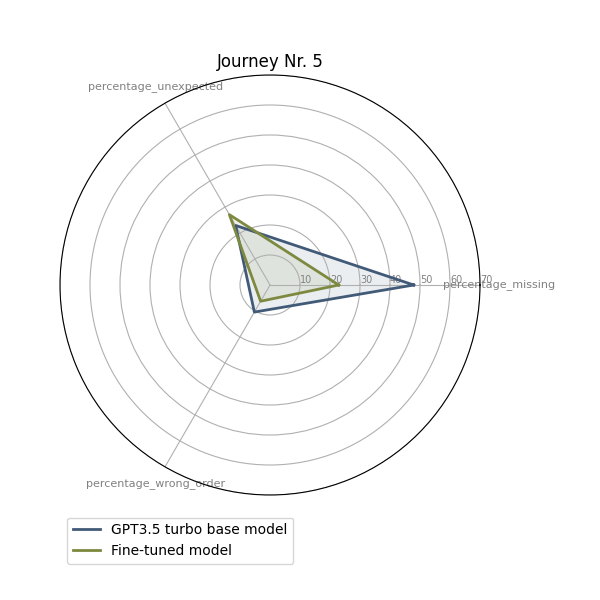
\includegraphics[width=0.3\textwidth]{bachelor_thesis/images/activites_pj5.png}}
  \caption{Comparison of GPT-3.5 Turbo and multi-task fine-tuned model for Patient Journey 1-5~\ref{apx:pjs} for the task \quotes{Activity Labelling}}
  \label{fig:eval_activities_rad}
\end{figure}
\paragraph{Activity Labelling} The plots in \autoref{fig:eval_activities_rad} show comparisons of the base model and multi-task fine-tuned model in all three metrics for each Patient Journey individually. The axes each display the error rate in the extraction results the models achieved. A smaller amplitude is desirable.\\
\autoref{fig:eval_activities_bar} illustrates the performance of both models across all patient journeys in a bar plot. Each bar represents the error rate in one of the metrics, and the bars of the same metric for each Patient Journey of base- and fine-tuned model overlap. A smaller amplitude is desirable. Although the fine-tuned model performed slightly worse in some metrics, its supremacy is evident. Especially with Patient Journey~1,2 and 4, the difference is clearly notable. We make the following observations:
\begin{enumerate}
    \item \emph{Wrong Order} is the error type with the least occurrences across both models. On average, there are more \emph{Missing Activity} errors than \emph{Unexpected Activity} errors. This indicates that both models tend to rather not include relevant events than include irrelevant or imaginary events.
    \item Patient Journey No.~5, which we assess as the most challenging, has the highest overall error rate. This hints at a correlation between lacklustre structure in Patient Journeys and worse event log quality.
    % \item The multi-task fine-tuned model overall outperforms the base model, though not consistently
\end{enumerate}

\begin{figure}[!htb]
    \centering
    \captionsetup{belowskip=0pt,aboveskip=0pt}
    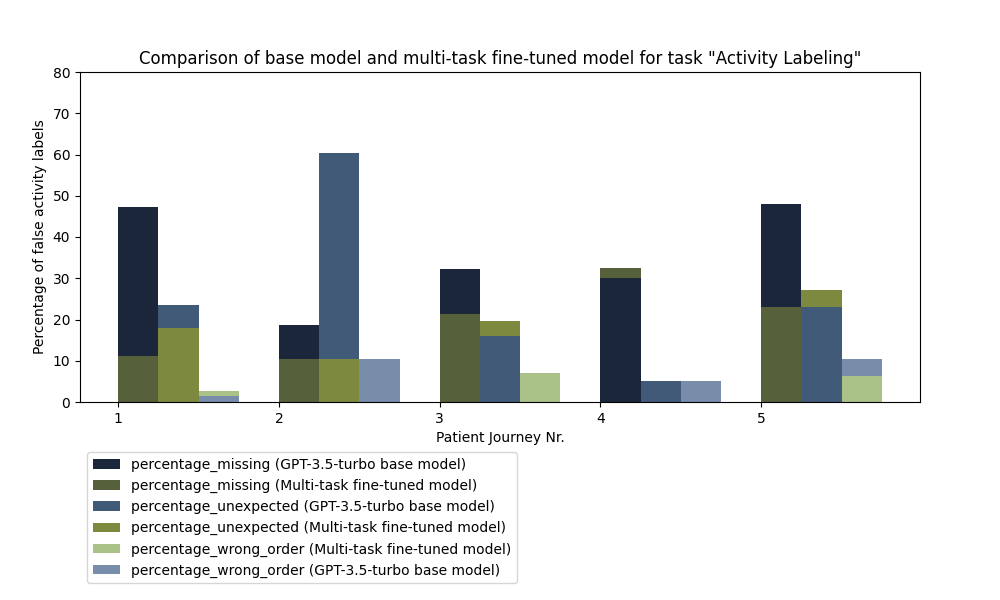
\includegraphics[width=\textwidth]{bachelor_thesis/images/activities_all.png}
    \caption{Comparison of GPT-3.5 Turbo and multi-task fine-tuned model across all Patient Journeys~\ref{apx:pjs} for the task \quotes{Activity Labelling}} 
    \label{fig:eval_activities_bar}
\end{figure}

\paragraph{Event Type Classification} \autoref{fig:eval_event_types} shows the performance of both models across all patient journeys in a bar plot. Each bar represents the percentage of incorrectly classified event types. GPT-3.5 Turbo performs better on three of the Patient Journeys. This can have various reasons, like an under-representation of certain event types in the training data. We discuss the matter in \autoref{sec:discussion}. The gap between the two models is relatively small, to a point where it can be almost considered negligible. Fine-tuning the model did not increase the quality of the extraction results in this task, for the majority of the measurements.
\begin{figure}[ht]
    \centering
    \captionsetup{belowskip=0pt,aboveskip=0pt}
    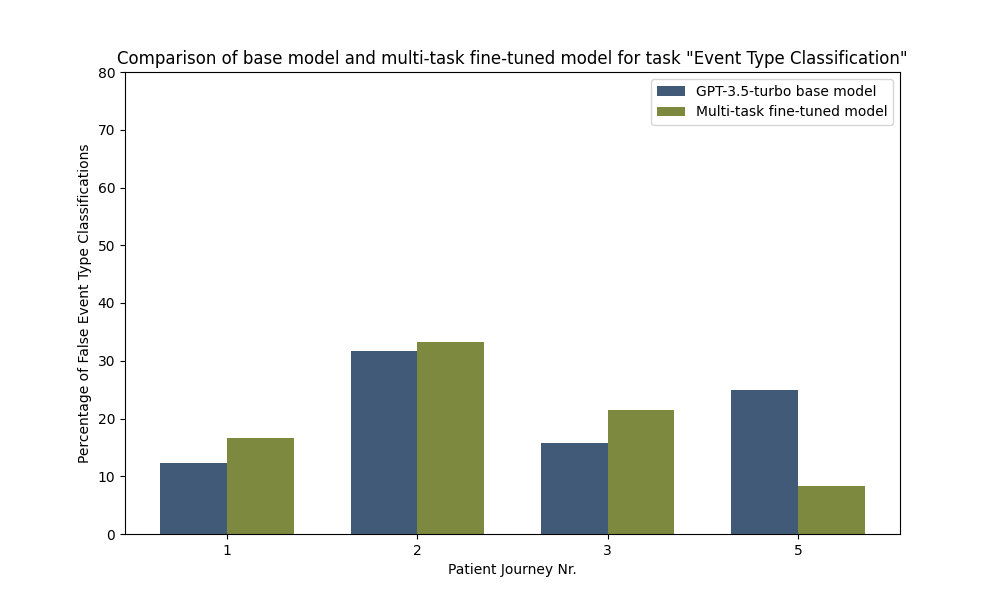
\includegraphics[width=\textwidth]{bachelor_thesis/images/event_types_all.png}
    \caption{Comparison of GPT-3.5 Turbo and multi-task fine-tuned model across all Patient Journeys~\ref{apx:pjs} for the task \quotes{Event Type Classification}}
    \label{fig:eval_event_types}
\end{figure}

\newpage
\paragraph{Timestamp Extraction}
The final task we trained the multi-task fine-tuned model for is extracting timestamps. \autoref{fig:eval_time} presents the ratio of incorrectly classified time stamps for GPT-3.5 Turbo and the fine-tuned model. A smaller amplitude is desirable. We make the following observations:
\begin{enumerate}
    \item The error rate in this metric is considerably higher than any other. This reflects our initial assessment that the extraction of timestamps is the most difficult task out of the ones we evaluate in this thesis.
    \item The multi-task fine-tuned model achieved a better quality in almost every scenario. Especially Patient Journey 1, 2 and 3 were processed noticeably better.
\end{enumerate}
Even the fine-tuned model struggles with less well-structured description of time specifications and events with strong temporal relations. Nevertheless, fine-tuning increases the quality of number of correctly extracted timestamps.
\begin{figure}[ht]
    \centering
    \captionsetup{belowskip=0pt,aboveskip=0pt}
    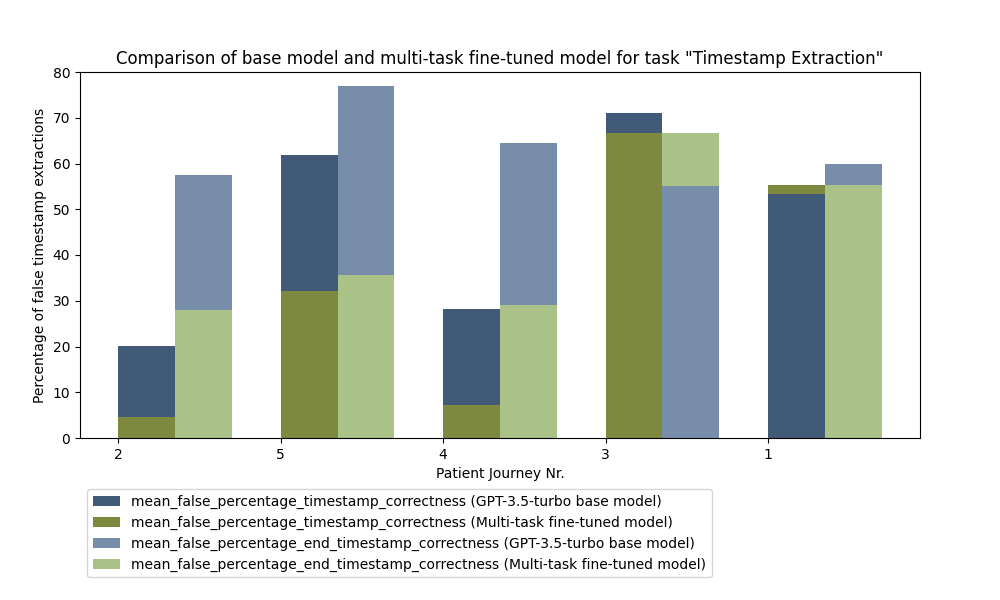
\includegraphics[width=\textwidth]{bachelor_thesis/images/timestamp_all.png}
    \caption{Comparison of GPT-3.5 Turbo and multi-task fine-tuned model across all Patient Journeys~\ref{apx:pjs} for the task \quotes{Timestamp Extraction}}
    \label{fig:eval_time}
\end{figure}


\subsubsection{Single-Task Fine-Tuned Model}\label{sec:eval_single} \vspace{-1em}
The plots in \autoref{fig:eval_activities_single_rad} show comparisons of the base model and single-task fine-tuned model in all three metrics for each Patient Journey individually. The axes each display the error rate in the extraction results the models achieved. A smaller amplitude is desirable.\\
\begin{figure}[p]
  \centering
  \captionsetup{belowskip=0pt,aboveskip=0pt}
  \subfigure[Patient Journey No. 1]{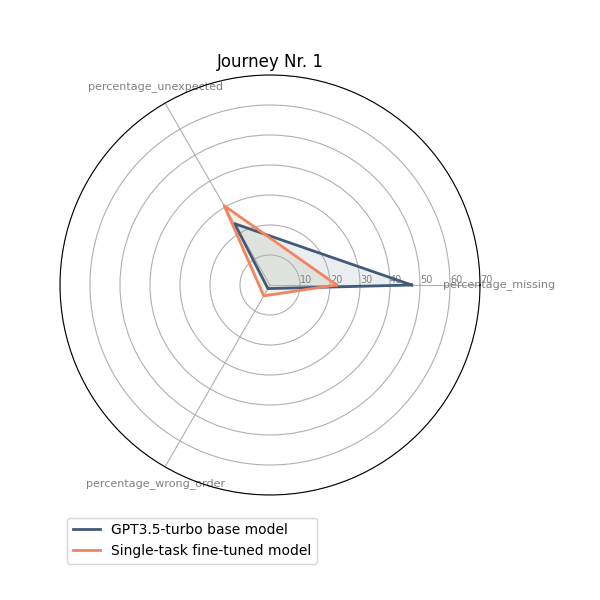
\includegraphics[width=0.3\textwidth]{bachelor_thesis/images/activites_pj1-single.png}}
  \subfigure[Patient Journey No. 2]{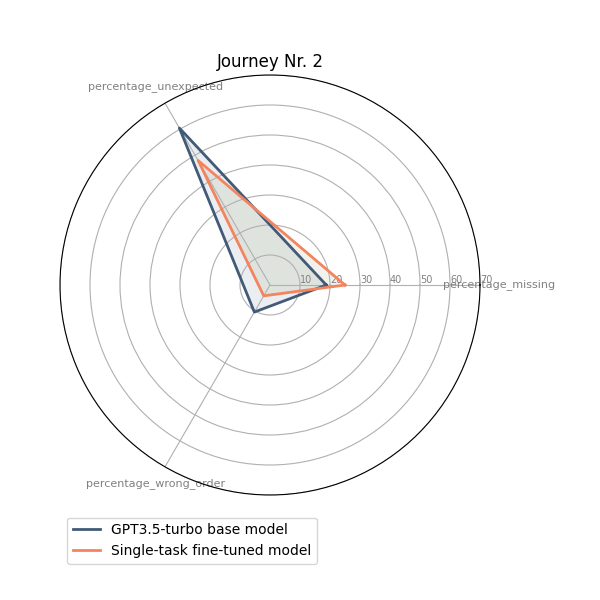
\includegraphics[width=0.3\textwidth]{bachelor_thesis/images/activites_pj2-single.png}}
  \subfigure[Patient Journey No. 3]{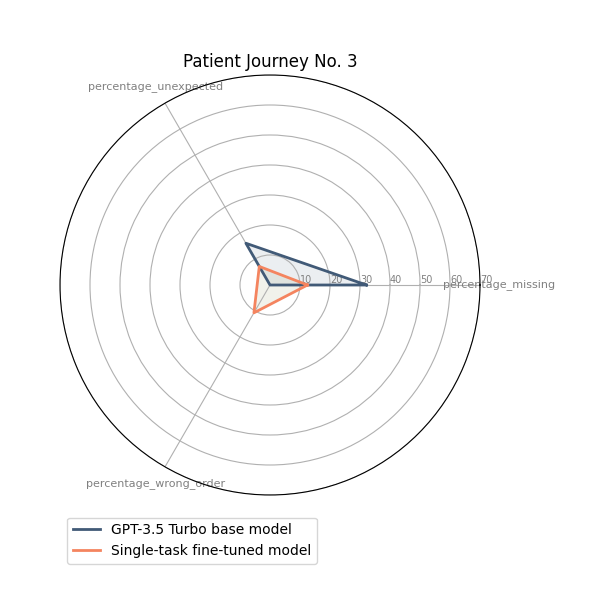
\includegraphics[width=0.3\textwidth]{bachelor_thesis/images/activites_pj3-single.png}}
  \subfigure[Patient Journey No. 4]{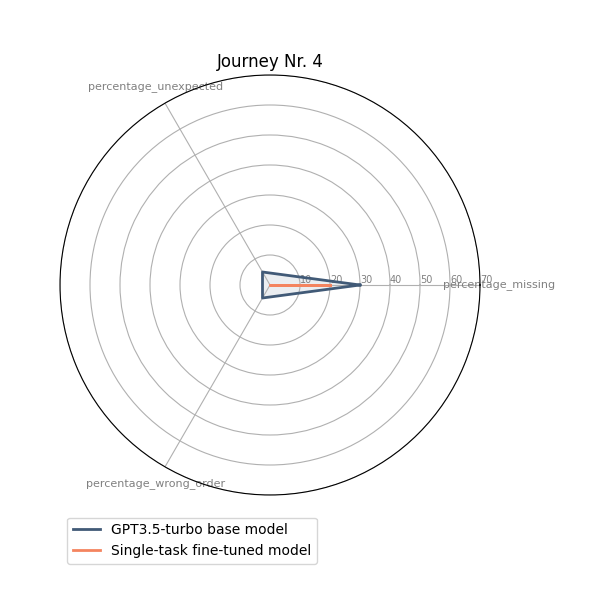
\includegraphics[width=0.3\textwidth]{bachelor_thesis/images/activites_pj4-single.png}}
  \subfigure[Patient Journey No. 5]{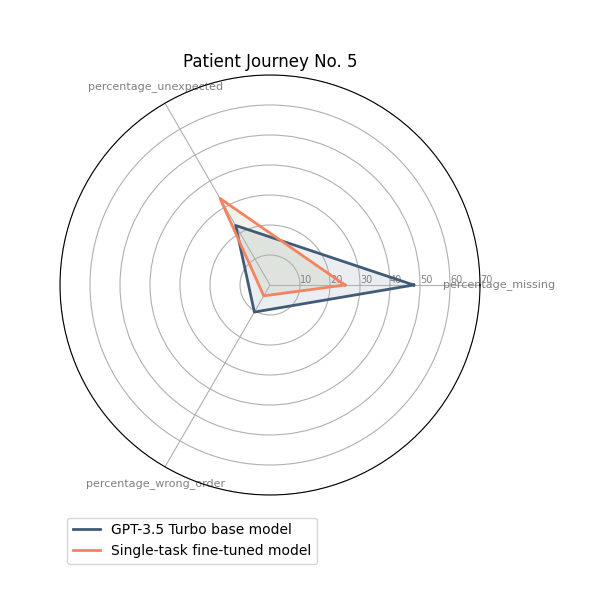
\includegraphics[width=0.3\textwidth]{bachelor_thesis/images/activites_pj5-single.png}}
  \caption{Comparison of GPT-3.5 Turbo and the Single-Task Fine-Tuned model for Patient Journey 1-5~\ref{apx:pjs} for the task \quotes{Activity Labelling}}
  \label{fig:eval_activities_single_rad}
\end{figure}
\autoref{fig:eval_activities_all_bar} illustrates the performance of both models across all patient journeys in a bar plot. Each bar represents the error rate in one of the metrics, and the bars of the same metric for each Patient Journey of base- and fine-tuned model overlap. A smaller amplitude is desirable. \\
The fine-tuned model consistently scores better in the \emph{missing activity} metric but only occasionally outperforms the base model in any other metric. 
\begin{figure}[hbt]
    \centering
    \captionsetup{belowskip=0pt,aboveskip=0pt}
    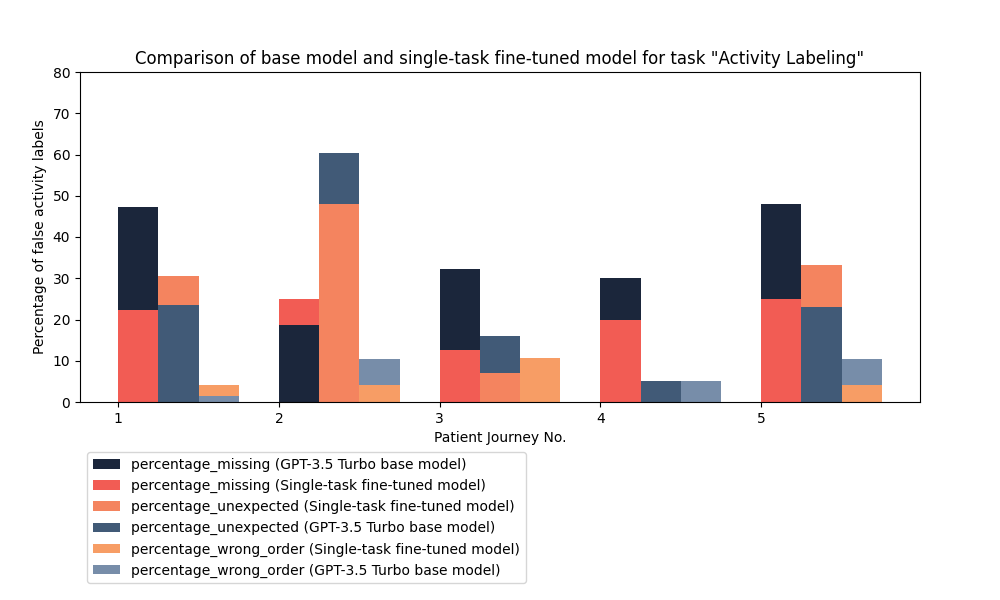
\includegraphics[width=\textwidth]{bachelor_thesis/images/activites_all-single.png}
    \caption{Comparison of GPT-3.5 Turbo and  Single-Task Fine-Tuned model across all Patient Journeys~\ref{apx:pjs} for the task \quotes{Activity Labelling}} 
    \label{fig:eval_activities_all_bar}
\end{figure}

\newpage
\subsubsection{Comparison of Fine-Tuned Models}
Lastly, we compare the results of the two fine-tuned models in their mutual task \quotes{Activity Labelling}. \autoref{fig:eval_activities_all_comparison_bar} shows that the multi-task fine-tuned model performs better in eight out of fifteen measurements, and the single-task fine-tuned model performs better in the other seven measurements. All models performed notably well on Patient Journey 3 and 4 for this task, indicating these are the easiest for an LLM to extract information from. The single-task fine-tuned model got the best scores for both of them. This indicates that the specialisation on one task increases the performance under easier conditions while not increasing the performance under more complex conditions. We further discuss this in~\autoref{sec:discussion}.

\begin{figure}[th]
    \centering
    \captionsetup{belowskip=0pt,aboveskip=0pt}
    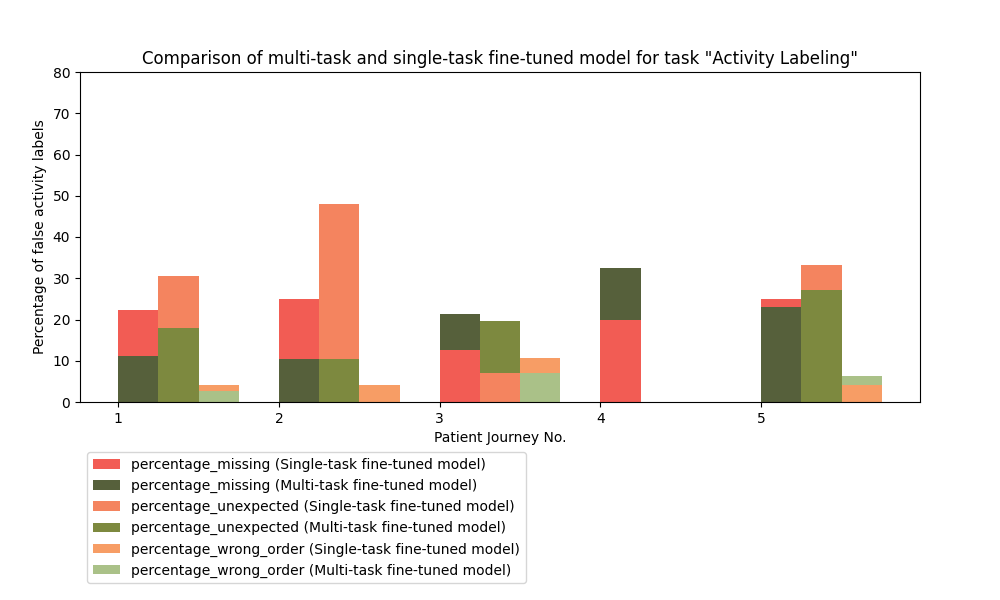
\includegraphics[width=\textwidth]{bachelor_thesis/images/activites_all-single_vs_multi.png}
    \caption{Comparison of multi-task and single-task fine-tuned model across all Patient Journeys~\ref{apx:pjs} for the task \quotes{Activity Labelling}} 
    \label{fig:eval_activities_all_comparison_bar}
\end{figure}
